\chapter{Dataset configuration management in MADTrack}\label{cap:Milestone1}

This chapter will cover the development of the features described in milestone 1 (codename \emph{D}), which is focused on the development of features related to Dataset
Configuration Management. This module will work in conjuction with the general configuration management module (see \emph{chapter \ref{cap:Milestone3}}) to provide mechanisms
to track and control the changes of the biggest of files. This chapter will introduce the main issues and address the problems to be solved to achieve the goals defined for this
milestone.

\section{Introduction}

One of the partial objectives defined for this Final Degree Project involves the development of a module for tracking and versioning datasets. These datasets can be of variable
size, but in many cases bigger than what a free-of-charge configuration management platform can handle. The lack of a platform that can handle such issue at
at a feasible cost motivates the creation of this dataset tracking module. The main focus of the prototypes of milestone 1 is to provide a mechanism for tracking changes within
datasets, without the need of committing them to the configuration management platform. Another issue to be tackled is that of bringing the correct dataset to the correct environment,
providing at least an interface for this purpose. Firstly, an analysis of the requirements defined for this milestone will be made, separating them by the most suitable
prototypes to be developed, and then proceeding to the development details of each of these.

\section{Requirements analysis for milestone 1}

Analysis has the purpose of defining the high-level outline of the application. The definition of this outline requires addressing the question of the most suitable architecture and
application type for the prototypes of this milestone. This analysis will also define the characteristics of a toolkit suitable for their development. Furthermore, the
protocol for versioning datasets will also be defined within the analysis phase.

\subsection{Requirements involved}

The requirements involved within this milestone have already been listed within \emph{table \ref{tab:requirementsMilestone1}}. Since this requirements are contained within different prototypes,
it is particularly convenient to define which requirements belong to which prototype. The final requirement division is defined within \emph{table \ref{tab:requirementsD1}} and \emph{table \ref{tab:requirementsD2}}.

Apart from the final requirement division for each prototype, all prototypes must satisfy the non-functional requirements listed within \emph{table \ref{tab:nonFunctionalRequirements}}.

\begin{table}[H]
    \centering
    \begin{tabular}{ | c | p{9cm} | p{3cm} |}
        \hline
        \textbf{Requirement ID} & \textbf{Requirement Description} & \textbf{priority (MoSCoW)} \\ \hline
        DFR1.2   & The system MUST keep track of the routes where models and datasets are stored    & Must have\\ \hline
    \end{tabular}
    \caption{Requirements for prototype \emph{D1}}
    \label{tab:requirementsD1}
\end{table}

\begin{table}[H]
    \centering
    \begin{tabular}{ | c | p{9cm} | p{3cm} |}
        \hline
        \textbf{Requirement ID} & \textbf{Requirement Description} & \textbf{priority (MoSCoW)} \\ \hline
		DFR1     & The system MUST keep ordered track of dataset configurations.                    & Must have\\ \hline
		DFR1.1   & The system MUST detect changes in the size (rows and columns) of datasets.       & Must have\\ \hline
    \end{tabular}
    \caption{Requirements for prototype \emph{D2}}
    \label{tab:requirementsD2}
\end{table}

\subsection{Integration with the rest of the system}

Prototypes within milestone 1 only have meaningful interaction with the general configuration management module, mainly because of their dependency on the committing and
checkout methods from milestone 3. 

\begin{figure}[H]
    \centering
    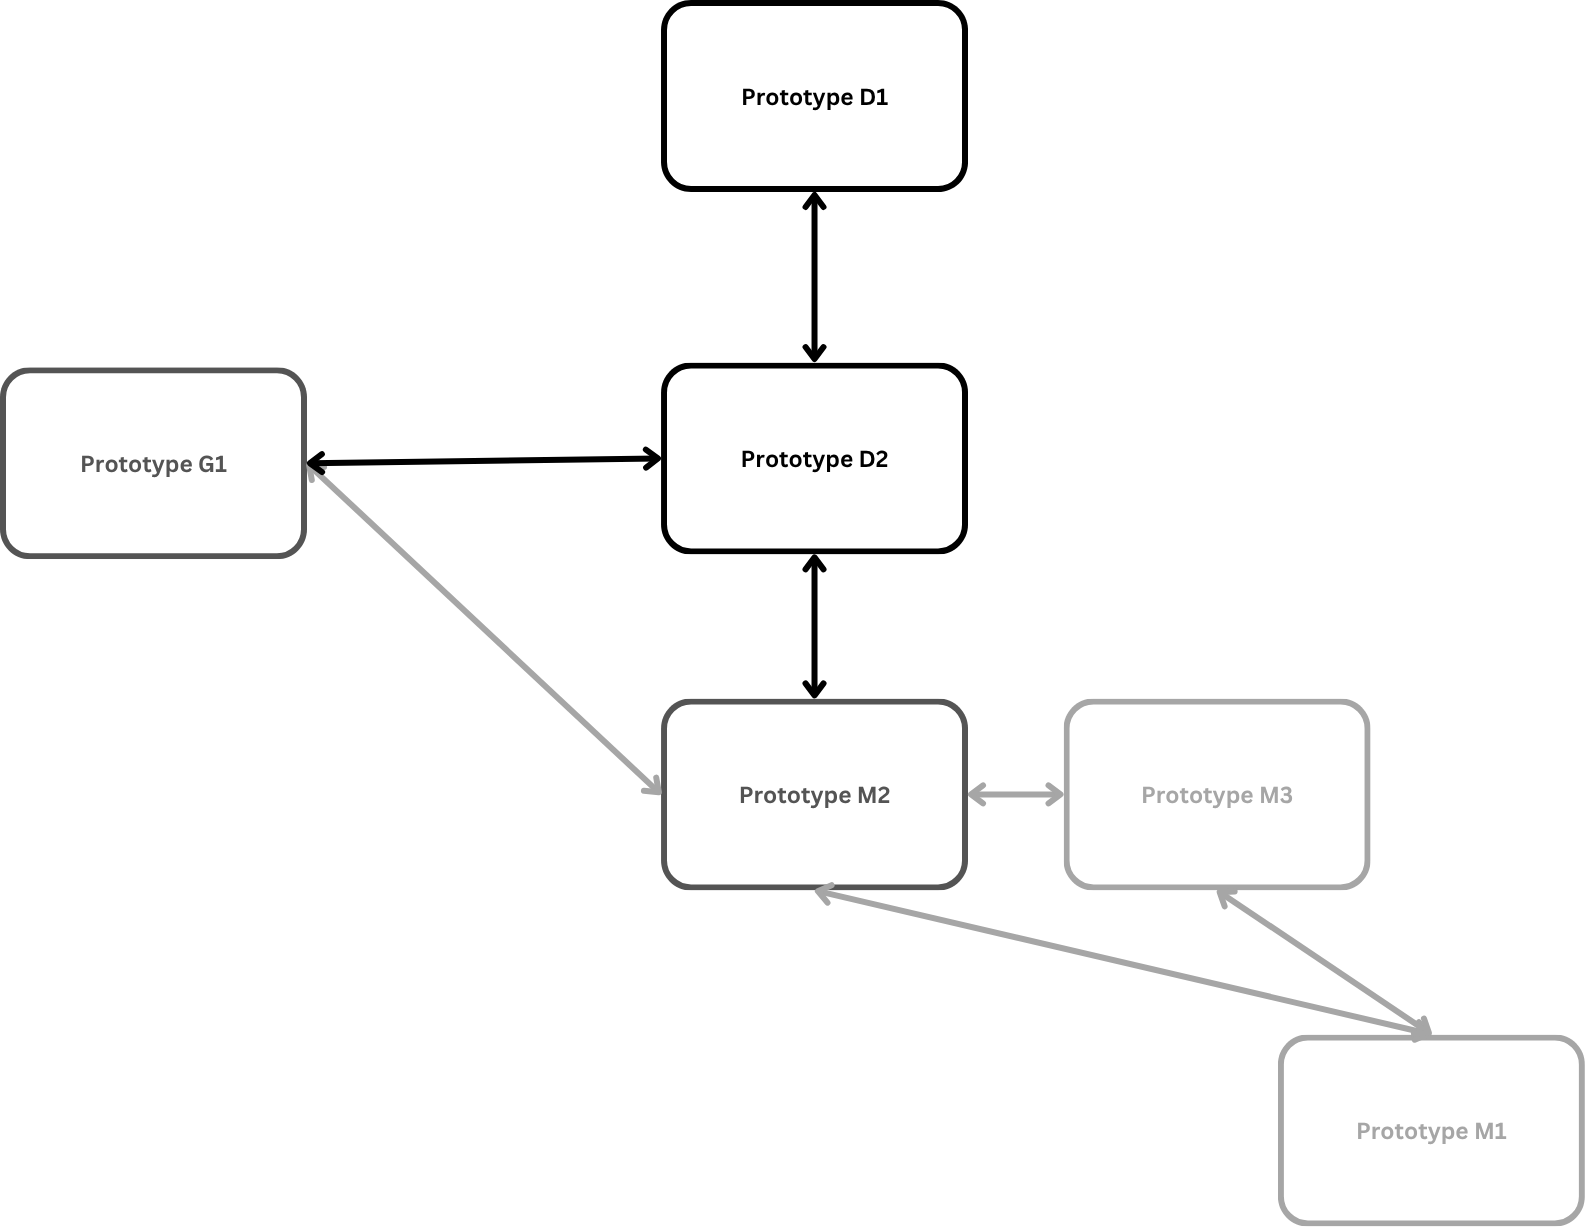
\includegraphics[width=0.7\textwidth]{figs/D-dependencies.png}
    \caption{Dependencies between prototypes of milestone 1 and the rest of the target system, shown by an interaction diagram.}
\end{figure}

\subsection{Architecture analysis}

The requirements describe the need for users to be able to locate files regarding datasets (and models, if it were necessary). Hence, an heterogeneous system will be 
required that is able to load a file or dataset from some sort of initial information, such as an URL. The architecture of this application will be monolithic, but will 
also have the capability to handle connections to remote file systems. Also, the upcoming prototypes will integrate an automatic version detection system that loads the file and 
sets it in the correct version.

\subsection{Application type analysis}

Since the main objective of this prototype is to locate and load files and perform configuration management operations on them, the most suitable application type is a Wrapper Library 
that covers online and local operations from a machine with authorized access to the file system.

\subsection{Toolkit analysis}

The most suitable toolkits that may serve for the development of this prototype are those related to dataset configuration management (from \emph{Chapter \ref{cap:StateOfTheArt}},
the tool with the most potential was DVC), a toolkit for accessing remote file systems securely and locating files within the local machine, and any toolkit providing a 
mechanism for changing between file versions (the Commit Manager component from prototype \emph{G1} of the system can be used for this purpose).

\subsection{Versioning protocol for datasets}\label{sec:versioningProtocol}

Any dataset integrated within MADTrack will be versioned using the following naming system:

\begin{table}[H]
    \centering
    \begin{tabular}{|c|}
        \hline
        \texttt{<dataset\_name> v<major\_version>.<minor\_version>} \\ \hline
    \end{tabular}
\end{table}

where:

\begin{itemize}
    \item \texttt{<dataset\_name>} is the name of the dataset.
    \item \texttt{<major\_version>} is a positive integer that represents major changes within the datasets without breaking semantics on the purpose of the dataset.
    \item \texttt{<minor\_version>} is a positive integer that represents minor changes within the datasets.
\end{itemize}

\section{Prototype design and development}

Within the coming sections, details for the design, implementation and testing phases of the development of this milestone's prototypes are shown in a sequential order. This
milestone is composed of two prototypes, whose development details will be shown in the following subsections.

\subsection{Prototype \emph{D1}}

Prototype D1 consists in the initial stage of development of milestone 1. The objective of this prototype is to 
provide the necessary mechanisms to integrate and transparently locate a dataset within the target system.

\subsubsection{Design for prototype \emph{D1}}

The use case diagram for prototype \emph{D1} is shown in \emph{figure \ref{fig:useCaseD1}}.

\begin{figure}[H]
    \centering
    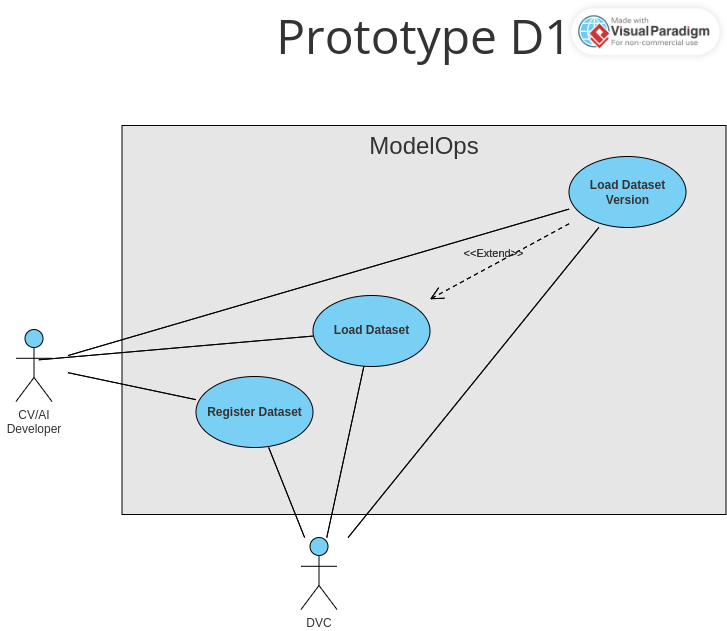
\includegraphics[width=0.7\linewidth]{figs/use-case-D1.png}
    \caption{Use case diagram for prototype \emph{D1}.}
    \label{fig:useCaseD1}
\end{figure}

Two main tasks can be extracted from this use case diagram. The first task is related to the tracking of changes within datasets, focusing particularly on enabling this action on a 
dataset. The second task, additionally, is to enable users to load datasets in either their latest version or any specific existent version. For the fulfillment of 
this objective, two new components will be created, along with a package with classes to represent exceptions, errors and specific states for a dataset repository.

\paragraph{Prototype \emph{D1} components}

\begin{itemize}
    \item \textbf{Dataset Tracker: }this component will be used for carrying out tasks related with tracking changes on the datasets. For this prototype, it should be 
    capable of starting the change tracking on a dataset and revert its state to a previous, past version.
    
    \item \textbf{Integration States: }an enumeration component that contains the possible states of integration of a dataset repository into ModelOps' configuration management 
    system: Fully integrated, partially or semi-integrated or not integrated.
    
    \item \textbf{Dataset Fetchers: }a series of components with the main purpose of providing users with the mechanism to obtain datasets from virtually any location, as well as to 
    load them in their different versions, by means of a unified interface to name the dataset versions. For this prototype, only one implementation of this interface will be made.
    
    \item \textbf{Dataset Exceptions: }a set of exceptions and errors created to represent the possible undesireable or exceptional states that can be encountered by operating 
    the previous two components.

\end{itemize}



\paragraph{Prototype \emph{D1} design output}\mbox{}\\

The design for prototype \emph{D1} is shown in \emph{Placeholder for annex figure}.

\subsubsection{Implementation for prototype \emph{D1}}

In the coming paragraphs, details for the tools used to implement this prototype are revealed.

\paragraph{Libraries} \mbox{}\\

The libraries used for the implementation of this prototype were:

\begin{itemize}
    \item \textbf{\emph{GitPython}: }this toolkit also helped in this prototype, as the Commit Manager has a synergy with the dataset configuration management module.
    \item \textbf{\emph{DVC}: }this library was used to implement the dataset integration and version change functionalities.
    \item \textbf{\emph{Logging}: }A library that enables the creation of log files and manages log operations within any Python application.
    \item \textbf{\emph{OS}: }this library returns for providing repository existence verification mechanisms.
    \item \textbf{\emph{SHutil}: }a library that enables the creation and removal of directories and files. mainly used for developing functionalities for the Local Dataset Fetcher component.
\end{itemize}

\subsubsection{Testing for prototype \emph{D1}}

This subsection contains information on the test suites and errors encountered during the testing phase of the prototype.

The test suites for this class can be found in \emph{annex reference placeholder}. % Referencia al Anexo con las tablas (porque pueden ser muy grandes y no es plan). Esto no es prioritario, puede esperar
In the same way, the errors encountered during the course of the testing phase of prototype \emph{G1} are shown in \emph{annex reference placeholder}. % De nuevo, esto puede esperar porque va al anexo

\subsection{Prototype \emph{D2}}

Prototype D2 is the second stage of development of Milestone 1. The objective of this prototype is to provide the necessary mechanisms to commit changes to a dataset.

\subsubsection{Design for prototype \emph{D2}}

The output of the design for prototype \emph{D2} is developed by designating the various components that make up this prototype, their contents and their connection with the rest of the system.
Hence, the design details for this prototype are shown in the following paragraphs.

\paragraph{Components for prototype \emph{D2}} \mbox{}\\

The use case diagram is shown in \emph{figure \ref{fig:useCaseD2}}.

\begin{figure}[H]
    \centering
    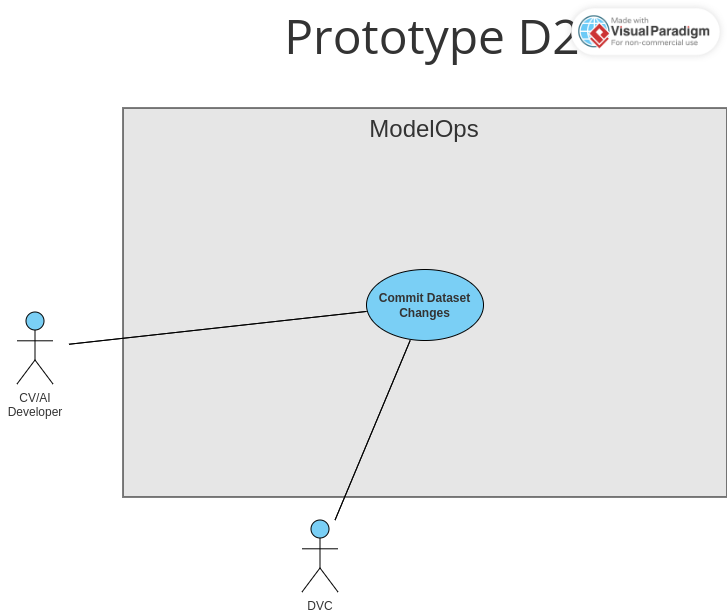
\includegraphics[width=0.7\linewidth]{figs/use-case-D2.png}
    \caption{Use case diagram for prototype \emph{D2}.}
    \label{fig:useCaseD2}
\end{figure}

The main task is to perform commits over a dataset. For this objective, the Dataset Tracker component can be used, as it already has a function that allows the user to 
commit changes to a dataset and generate a new version of it. Hence, the involved components are:

\begin{itemize}
    \item \textbf{Dataset Tracker: }this class will be used for carrying out tasks related with tracking changes on the datasets. For this prototype, it should be capable of creating new versions of a dataset and upload them to a local or remote repository.
\end{itemize}

\paragraph{Design output for prototype \emph{D2}}\mbox{}\\

The design class diagram for prototype D2 is shown in \emph{Placeholder for annex figure}.

\subsubsection{Implementation for prototype \emph{D2}}

Prototype \emph{D2} mostly follows the same implementation details as the previous prototype of the milestone. Following Python as the main programming language and the same
libraries.

\subsubsection{Testing for prototype \emph{D2}}

The testing phase of prototype \emph{D2} was clearly focused on testing the new methods. Since the method \texttt{getCurrentDatasetName} is a read-only 
method that just calls the Commit Manager, its testing can be omitted. The test suites of the remaining method can be found at \emph{annex reference placeholder} and the errors fixed can be found at \emph{annex reference placeholder}.

\paragraph{Test suites for prototype \emph{D2}}\mbox{}\\

The test suites for this class can be found in \emph{annex reference placeholder}.

\paragraph{Errors found and lessons learned during the development of prototype \emph{D2}}\mbox{}\\

The errors encountered during the course of the testing phase of prototype \emph{D2} are shown in \emph{annex reference placeholder}.

